\section{Linux e exemplos de utilização} \label{section: linux e exemplos}

\subsection{História}
O \textbf{GNU/Linux} é um sistema operativo \textit{open source}, criado por \textbf{Linus Torvalds} em 1991 após a sua exposição inicial a sistemas \textbf{Unix} enquanto estudante de informática na Universidade de Helsínquia, na Finlândia.
\par \vspace{6pt}
O nome \textbf{Linux} é uma combinação do primeiro nome de seu criador, \textbf{Linus}, e do sistema operativo \textbf{Unix}, que serviu de inspiração para os seus projetos. Na altura, a maioria dos sistemas operativos era proprietária e cara, levando Linus a decidir criar um sistema operativo que estivesse disponível gratuitamente para qualquer pessoa. \cite{linuxHistory}
\par \vspace{6pt}
O Projeto \textbf{GNU}, liderado por \textbf{Richard Stallman} desde 1983, é fundamental para a história do Linux. Ao oferecer um conjunto completo de ferramentas e utilitários de software livre, o \textbf{GNU} forneceu a base essencial para várias distribuições Linux. Além disso, o \textbf{GNU} também contribuiu para a nomenclatura oficial, dando origem ao nome \textbf{GNU/Linux}. Essa colaboração entre o \textbf{GNU} e o kernel \textbf{Linux} resultou em sistemas operativos mais robustos e na capacidade de manter o GNU/Linux completamente livre. \cite{gnuHistory}
\par \vspace{6pt}
As primeiras versões do GNU/Linux eram principalmente utilizadas por entusiastas da tecnologia e desenvolvedores de software. Com o passar do tempo, a sua popularidade cresceu rapidamente, levando à sua adoção em uma ampla gama de ambientes.
\par \vspace{6pt}
O GNU/Linux é reconhecido como um dos sistemas operativos mais estáveis, seguros e confiáveis, sendo amplamente adotado em \textbf{servidores}, \textbf{supercomputadores} e \textbf{ambientes empresariais}. Com o crescimento de sua popularidade e o contínuo desenvolvimento pela comunidade, hoje, algumas das principais distribuições GNU/Linux incluem o \textbf{Ubuntu, Fedora, Arch, Red Hat, Debian, Mint} e \textbf{Manjaro}.

\par \vspace{13pt}

\begin{figure}[H]
    \centering
    % width=\textwidth para imagem da largura do texto
    
\includegraphics[scale=2.8]{Figures/0. General/linux_distros.png}
    \caption{Tipos de distribuições ou "distros" de linux}
    \label{Distros de linux}
\end{figure}

\newpage
\subsection{Presença em diversos ambientes}
O GNU/Linux está presente em uma ampla variedade de ambientes, incluindo: \cite{diverseUsage}
\begin{itemize}

    \item \textbf{Servidores e data centers}\\
    O GNU/Linux é amplamente reconhecido pelo seu domínio no mercado de servidores e centros de dados, destacando-se pela sua estabilidade e confiabilidade. É frequentemente utilizado para operar \textbf{redes de dados} e \textbf{data centers}.

    Muitos dos equipamentos constituintes dos servidores e data centers, tais como os \textbf{routers}, funcionam com versões personalizadas e simplificadas do sistema operativo GNU/Linux.

    \item \textbf{Supercomputadores}\\
    A capacidade do GNU/Linux para escalar eficientemente até milhares de núcleos de processamento, aliada à sua flexibilidade para otimização em tarefas de alto desempenho, são características essenciais para o seu uso em supercomputadores. 
    
    Na verdade, o GNU/Linux é o sistema operativo preferido para a maioria dos supercomputadores, evidenciando a sua eficiência em ambientes de computação intensiva.
    
    \item \textbf{Dispositivos IoT}\\
    No âmbito da \textbf{Internet das Coisas (IoT)}, o GNU/Linux destaca-se devido ao seu tamanho compacto e à sua capacidade de adaptação para se adequar a hardware específico. Desde \textbf{eletrodomésticos inteligentes} até sistemas avançados de \textbf{controlo industrial} e \textbf{veículos autónomos}, o GNU/Linux serve como uma base fiável para uma variedade de dispositivos inovadores.

    \item \textbf{Desktops e uso diário}\\
    Embora seja menos popular que o \textbf{Windows} ou o \textbf{MacOS} em desktops, o GNU/Linux tem observado um aumento constante na sua aceitação por parte dos utilizadores. Esta tendência deve-se à sua crescente biblioteca de programas de software baseados em GNU/Linux e a um foco contínuo na expansão da oferta de interfaces de utilizador mais amigáveis para desktop. Além disso, o sistema operativo GNU/Linux serve como a base de outros sistemas operativos amplamente utilizados no nosso quotidiano, como o \textbf{Android} e o \textbf{Chrome OS}.

    \item \textbf{Educação e governo}\\
    O GNU/Linux é altamente valorizado por instituições educativas e governamentais devido ao seu baixo custo e à sua capacidade de personalização. Em todo o mundo, vários governos têm implementado extensivamente o GNU/Linux nas operações governamentais e nos sistemas educacionais, aproveitando essas vantagens.
\end{itemize}

\par \vspace{6pt}

\begin{figure}[H]
    \centering
    % width=\textwidth para imagem da largura do texto
    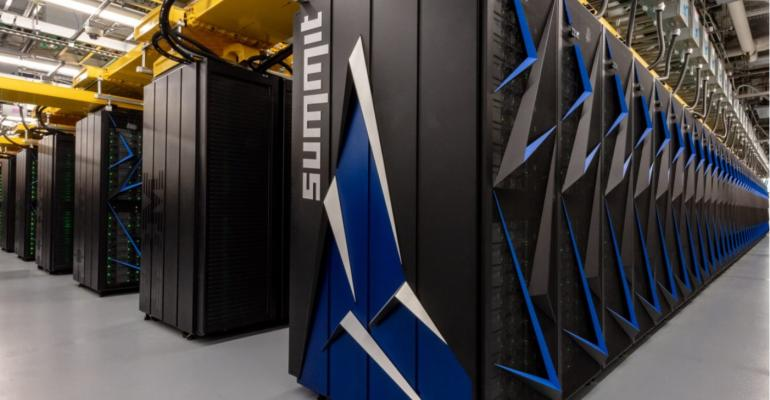
\includegraphics[scale=0.4]{Figures/0. General/super_computer.jpg}
    \caption{Supercomputador da IBM a correr Linux}
    \label{Supercomputador da IBM a correr Linux}
\end{figure}